%%%%%%%%%%%%%%%%%%%%%%%%%%%%%%%%%%%%%%%%%%%%%%%%%%%%%%%%%%%%%%%%%%%%%%%%%%%%%%%%%%%%%%%%%%%%%%%%
%
% CS484 Written Question Template
%
% Acknowledgements:
% The original code is written by Prof. James Tompkin (james_tompkin@brown.edu).
% The second version is revised by Prof. Min H. Kim (minhkim@kaist.ac.kr).
%
% This is a LaTeX document. LaTeX is a markup language for producing 
% documents. Your task is to fill out this document, then to compile 
% it into a PDF document. 
%
% 
% TO COMPILE:
% > pdflatex thisfile.tex
%
% If you do not have LaTeX and need a LaTeX distribution:
% - Personal laptops (all common OS): www.latex-project.org/get/
% - We recommend latex compiler miktex (https://miktex.org/) for windows,
%   macTex (http://www.tug.org/mactex/) for macOS users.
%   And TeXstudio(http://www.texstudio.org/) for latex editor.
%   You should install both compiler and editor for editing latex.
%   The another option is Overleaf (https://www.overleaf.com/) which is 
%   an online latex editor.
%
% If you need help with LaTeX, please come to office hours. 
% Or, there is plenty of help online:
% https://en.wikibooks.org/wiki/LaTeX
%
% Good luck!
% Min and the CS484 staff
%
%%%%%%%%%%%%%%%%%%%%%%%%%%%%%%%%%%%%%%%%%%%%%%%%%%%%%%%%%%%%%%%%%%%%%%%%%%%%%%%%%%%%%%%%%%%%%%%%
%
% How to include two graphics on the same line:
% 
% \includegraphics[width=0.49\linewidth]{yourgraphic1.png}
% \includegraphics[width=0.49\linewidth]{yourgraphic2.png}
%
% How to include equations:
%
% \begin{equation}
% y = mx+c
% \end{equation}
% 
%%%%%%%%%%%%%%%%%%%%%%%%%%%%%%%%%%%%%%%%%%%%%%%%%%%%%%%%%%%%%%%%%%%%%%%%%%%%%%%%%%%%%%%%%%%%%%%%

\documentclass[11pt]{article}

\usepackage[english]{babel}
\usepackage[utf8]{inputenc}
\usepackage[colorlinks = true,
linkcolor = blue,
urlcolor  = blue]{hyperref}
\usepackage[a4paper,margin=1.5in]{geometry}
\usepackage{stackengine,graphicx}
\usepackage{fancyhdr}
\setlength{\headheight}{15pt}
\usepackage{microtype}
\usepackage{times}

% From https://ctan.org/pkg/matlab-prettifier
\usepackage[numbered,framed]{matlab-prettifier}

\frenchspacing
\setlength{\parindent}{0cm} % Default is 15pt.
\setlength{\parskip}{0.3cm plus1mm minus1mm}

\pagestyle{fancy}
\fancyhf{}
\lhead{Homework 2 Questions}
\rhead{CS484}
\rfoot{\thepage}

\date{}

\title{\vspace{-1cm}Homework 2 Questions}


\begin{document}
	\maketitle
	\vspace{-3cm}
	\thispagestyle{fancy}
	
	\section*{Instructions}
	\begin{itemize}
		\item 4 questions.
		\item Write code where appropriate.
		\item Feel free to include images or equations.
		\item \textbf{Please use only the space provided and keep the page breaks.} Please do not make new pages, nor remove pages. The document is a template to help grading.
		\item If you really need extra space, please use new pages at the end of the document and refer us to it in your answers.
	\end{itemize}

	\section*{Questions}
	
	\paragraph{Q1:} Explicitly describe image convolution: the input, the transformation, and the output. Why is it useful for computer vision?
	
	%%%%%%%%%%%%%%%%%%%%%%%%%%%%%%%%%%%
	\paragraph{A1:} Your answer here.
	\\ \\
	Convolution is image processing by using a filter. Convolution takes 2 inputs, a image(I) and a filter(f) and transforms them. Filter (kernel) is the matrix which is operated to the image. The transformation is expressed in the equation below.\\

	\begin{figure}[h]
    \centering
    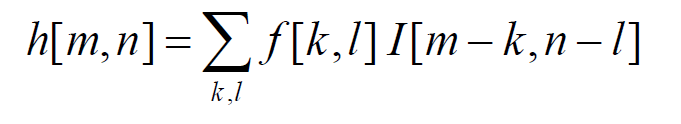
\includegraphics[width=5cm]{questions/convolution.PNG}
    \label{fig:equation1}
    \end{figure}
    
    Here, the image and filter are both in 2D. If the image I is colored, h[m,n,k] (k is color dimension) can be calculated by using above equation for R, G, B respectively. The output is the image(h) which is an image after filtering(transformed) by 'f'. Convolution is important because it has a lot of useful mathmetical properties such as shift invariance, commutativity, and associativity, which make image filtering comfortable and applicable. 
	
	
	
	
	%%%%%%%%%%%%%%%%%%%%%%%%%%%%%%%%%%%
	
	% Please leave the pagebreak
	\pagebreak
	\paragraph{Q2:} What is the difference between convolution and correlation? Construct a scenario which produces a different output between both operations.
	
	\emph{Please use \href{https://www.mathworks.com/help/images/ref/imfilter.html}{$imfilter$} to experiment! Look at the `options' parameter in MATLAB Help to learn how to switch the underlying operation from correlation to convolution.}
	
	%%%%%%%%%%%%%%%%%%%%%%%%%%%%%%%%%%%
	\paragraph{A2:} Your answer here.
    \\ 	
    Correlation's definition is below.
    \begin{figure}[h]
    \centering
    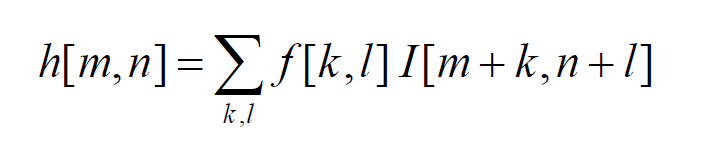
\includegraphics[width=5cm]{questions/correlation.PNG}
    \label{fig:equation2}
    \end{figure}
    
    From the convolution equation in A1, they are different only in terms of addition and subtraction. Thus, there are some properties that convolution has but correlation doesn't, such as commutativity. However, correlation and convolution are identical only when the filter is origin symmetric.\\
    
    \begin{lstlisting}[style=Matlab-editor]
    A = imread('../data/cat.bmp');
    filter = [1,1,1;0,0,0;-1,-1,-1];
    
    A1 = imfilter(A, filter);
    A2 = imfilter(A, filter, 'conv');
    \end{lstlisting}
    
	\begin{figure}[h]
    \centering
    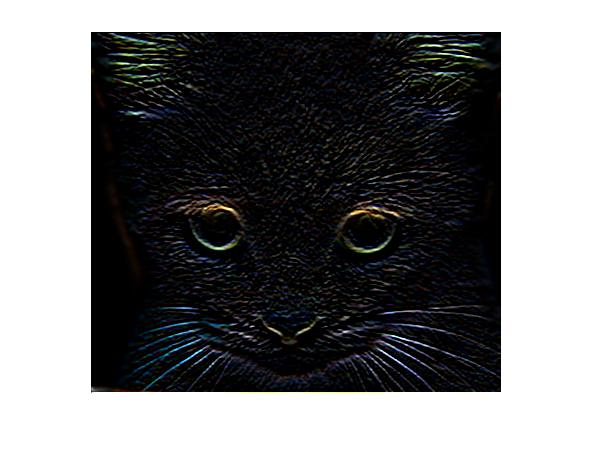
\includegraphics[width=6cm]{questions/f1.jpg}
    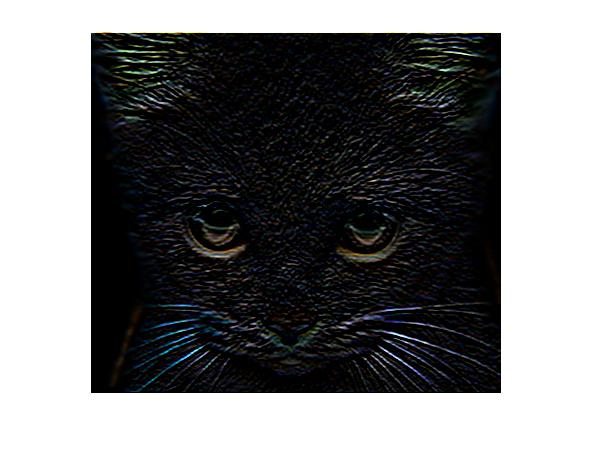
\includegraphics[width=6cm]{questions/f2.jpg}
    \caption{\emph{Left:} A1, \emph{Right:} A2}
    \end{figure}
	
	In the code, 'filter' is not origin symmetry. So, the results of imfilter(A, filter) (correlation) and imfilter(A, filter, 'conv') (convolution) are different. 
	
	
	%%%%%%%%%%%%%%%%%%%%%%%%%%%%%%%%%%%
	
	% Please leave the pagebreak
	\pagebreak
	\paragraph{Q3:} What is the difference between a high pass filter and a low pass filter in how they are constructed, and what they do to the image? Please provide example kernels and output images.
	
	%%%%%%%%%%%%%%%%%%%%%%%%%%%%%%%%%%%
	\paragraph{A3:} Your answer here.\\
	
	High pass filter cut off the low frequencies of the image when doing convolution, while low pass filter cut off the high frequencies. Using Gaussian filter, we can cut off the high frequencies of the image. Also, we can cut off the low frequencies by simply subtracting the low frequencies-passed image from its original image, or using Laplacian filter. High-cut filter smooth the image with the outline blurred, and low-cut filter highlight the outline and other values make negative (black).\\
	high pass filter example: [-1/8,-1/8,-1/8;-1/8,1,-1/8;-1/8,-1/8,-1/8];\\
	low pass filter example: [1/9,1/9,1/9;1/9,1/9,1/9;1/9,1/9,1/9];
	
	\begin{lstlisting}[style=Matlab-editor]
    %Standard deviation of the Gaussian blur.
    cutoff_frequency = 2.5;
    
    %low pass filter (Gaussian)
    lowpassfilter = fspecial('Gaussian', cutoff_frequency*4+1, cutoff_frequency);
    
    %high pass filter (subtract Gaussian from original image)
    [X, Y] = size(lowpassfilter);
    highpassfilter = zeros([X, Y]);
    highpassfilter((X-1)/2 + 1, (Y-1)/2 + 1) = 1;
    highpassfilter = highpassfilter - lowpassfilter;
	\end{lstlisting}
	\begin{figure}[h]
    \centering
    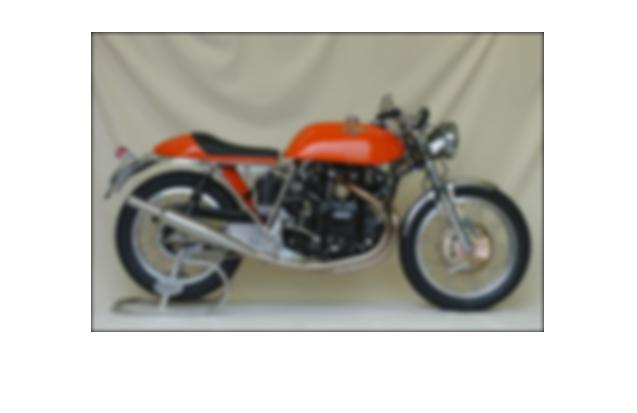
\includegraphics[width=5cm]{questions/low_frequencies1.jpg}
    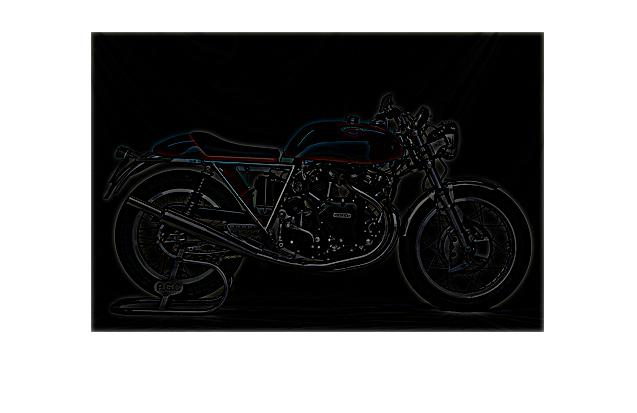
\includegraphics[width=5cm]{questions/high_frequencies1.jpg}
    \caption{\emph{Left:} image of low frequencies,\emph{Right:} image of high frequencies}
    \end{figure}
	
	
	%%%%%%%%%%%%%%%%%%%%%%%%%%%%%%%%%%%
	
	% Please leave the pagebreak
	\pagebreak
	\paragraph{Q4:} How does computation time vary with filter sizes from $3\times3$ to $15\times15$ (for all odd and square sizes), and with image sizes from 0.25~MPix to 8~MPix (choose your own intervals)? Measure both using \href{https://www.mathworks.com/help/images/ref/imfilter.html}{$imfilter$} to produce a matrix of values. Use the \href{https://www.mathworks.com/help/images/ref/imresize.html}{$imresize$} function to vary the size of an image. Use an appropriate charting function to plot your matrix of results, such as \href{https://www.mathworks.com/help/matlab/ref/scatter3.html}{$scatter3$} or \href{https://www.mathworks.com/help/matlab/ref/surf.html}{$surf$}.
	
	Do the results match your expectation given the number of multiply and add operations in convolution?
	
	See RISDance.jpg in the attached file.
	
	%%%%%%%%%%%%%%%%%%%%%%%%%%%%%%%%%%%
	\paragraph{A4:} Your answer here.
	\\ I used scale for image from 0.03 to 1.03, with interval of 0.1, and 'eye' function as filter. The result is below.
	\begin{figure}[h]
    \centering
    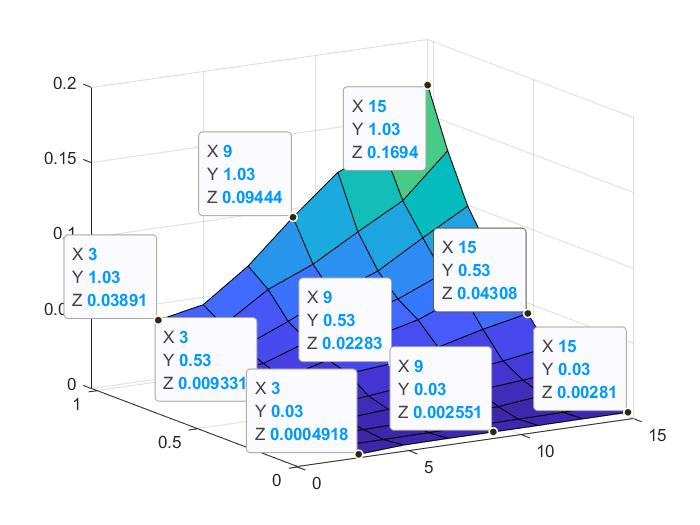
\includegraphics[width=10cm]{questions/surf.jpg}
    \caption{ X: size of kernel's sides, Y: scale of resized image, Z: time to implement 'imfilter'.}
    \end{figure}
	\\It seems that the time is $$O(X*Y^2)$$\\
	I expected that the time should be  $$O(X*Y)$$  because imfilter do seperation of column and row in this case. However, I don't know why it takes Y square, because Y is the scale of the image, not the scale of one side of image. I think it occurs because of wrong regression, or Matlab methods' time redundancies.
	
	%%%%%%%%%%%%%%%%%%%%%%%%%%%%%%%%%%%
	
	
	% If you really need extra space, uncomment here and use extra pages after the last question.
	% Please refer here in your original answer. Thanks!
	%\pagebreak
	%\paragraph{AX.X Continued:} Your answer continued here.
	
	
	
\end{document}